\section{Case Study: Spacecraft Rendezvous Passive Safety}
\label{sec:casestudy}

We evaluate our method on a spacecraft rendezvous passive safety case study.
%
The system consists of a primary chaser spacecraft moving towards a secondary, free-flying object (such as a satellite) and performing close-proximity maneuvers.
%
The maneuver is analyzed in relative coordinates, as shown in Figure~\ref{fig:chaser}.
%
The verification goal is to ensure \emph{passive safety}: at any time in the maneuver, a system failure may occur and the resulting propulsion-free trajectory must avoid colliding with the target satellite.
%
This requirement comes from real-world failures. In 2005, NASA's DART spacecraft was intended to rendezvous with the MUBLCOM satellite, but due to depleted propellant instead collided with the target satellite (a loss of a
\$110 million project)~\cite{croomes2006overview}.

\begin{figure}[t]
\centerline{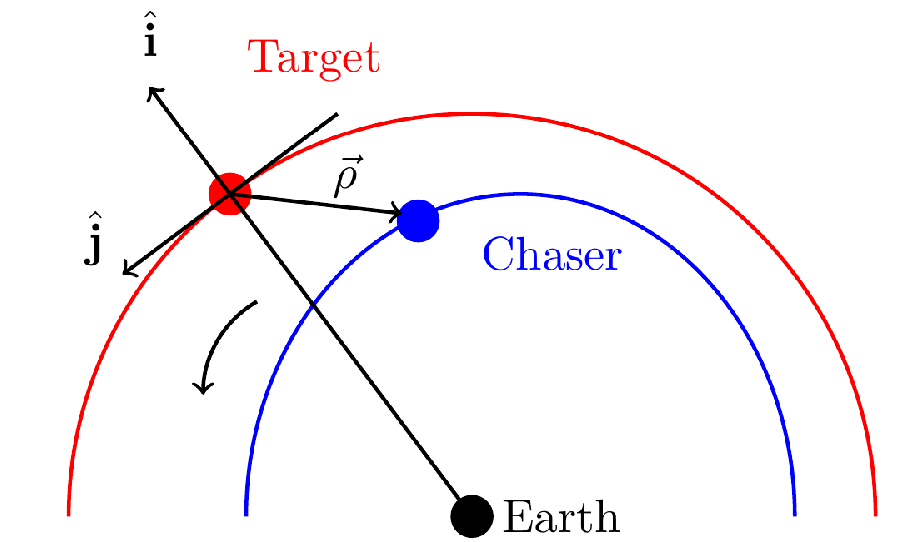
\includegraphics[width=0.5\columnwidth]{images/chaser.png}}
\caption{Collisions are checked between spacecraft in orbit in relative coordinates (image from~\cite{chan2017verifying}).}
\label{fig:chaser}
\end{figure}


Our model is based on a published spacecraft rendezvous benchmark~\cite{chan2017verifying,jewison2016spacecraft}.
%
The system is modeled as a hybrid automaton with different discrete modes depending on the sensors being used for navigation, and an LQR controller is designed to meet physical and geometric safety constraints.
%
The relative dynamics are linearized using the Clohessy-Wiltshire-Hill (CWH) equations~\cite{wh1960terminal},
which is often used in close proximity operations, and generally considered valid when spacecraft are within a few kilometers.
%
The hybrid automaton consists of three modes, two for different navigation strategies, and one for the passive dynamics, shown in Figure~\ref{fig:ha}.
%
This system is a six-dimensional linear system, with nondeterministic transitions to the passive mode.
%
In our analysis, we check for passive safety from $t_1=0$ to $t_2=250$.
%
The dynamics and controller in each mode are as described in the benchmark paper~\cite{chan2017verifying}.
%
We also use the same initial set of states, the box where $x \in [-925, -875]$, $y \in [-425, -375]$ and the velocities are zero.
%
We focus on the collision-free safety requirement, and strive to verify that the spacecraft remain separated by at least
5 meters in the infinity norm (the unsafe set is a $10 \times 10$ box centered at the origin).

Although several tools have successfully analyzed a version of this model in the ARCH hybrid systems tools competition in
2018~\cite{archcomp18linear}, a critical simplification was made: the competition model did not actually check the passive safety requirement.
%
In particular, the competition model used a \emph{fixed} time to transition to the passive mode.
%
This is an unrealistic simplification, since the time of failure cannot not be known in advance.


The analysis done in the original work~\cite{chan2017verifying} is slightly better, in that it checks for passive safety for a known 5 minute failure interval.
%
In~\cite{chan2017verifying}, the author that, if larger time intervals are used,
``the initial set of states under the Passive mode is large, making it very difficult to prove safety.''
%
The suggestion is then to create subintervals that cover the full time range of transitions to the passive mode, and then successively
analyze each interval as a standalone verification problem.
%
Presumably, a manual guess-and-check approach should be used to create these subintervals.

\begin{figure}[t]
\centerline{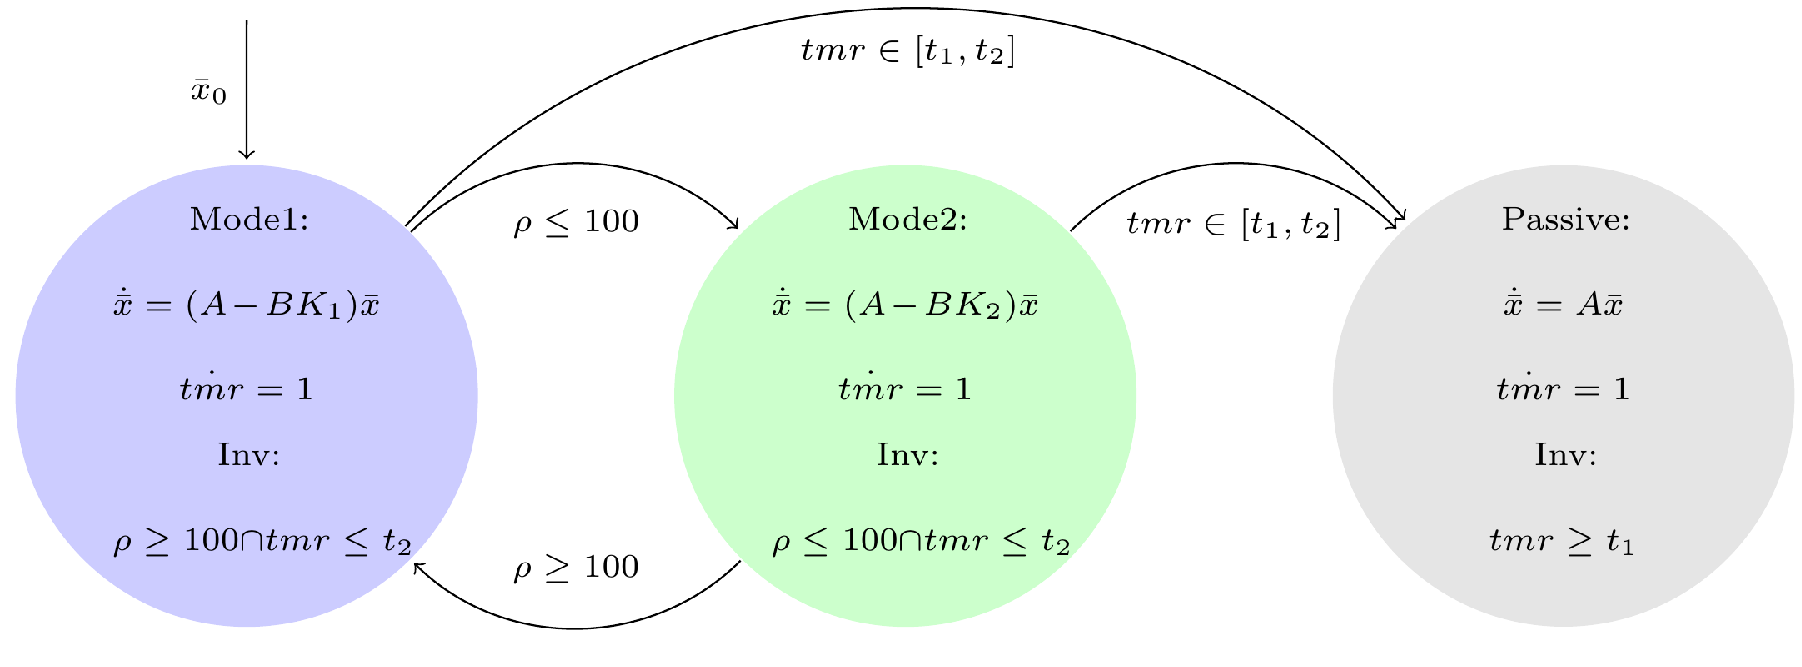
\includegraphics[width=0.9\columnwidth]{images/ha.png}}
\caption{Hybrid automaton model for our case study (image from~\cite{chan2017verifying}, which also include the dynamics matrices). We check for passive safety
  from time $t_1=70 - r$ to $t_2=70 + r$, where $r$ is a model parameter.}
\label{fig:ha}
\end{figure}

We consider a parameterized version of the problem, where a single parameter $r$ controls the amount of nondeterminism in the switch to the passive mode.
%
A simulation-based analysis revealed that entering the passive mode up to around time 140 will not violate the collision safety specification.
%
We thus consider enable the switch to the passive mode from time $70-r$ to time $70+r$.
%
In this way, $r=0$ corresponds to the easy case where the switch
occurs at exactly time $70$, and $r=70$ corresponds to the difficult case where the switch can occur at any time between $0$ and $140$.
%
In the automaton in Figure~\ref{fig:ha}, we set $t_1=70 - r$ and $t_2=70 + r$.

All the experiments are performed on a system with an Intel i5-5300U CPU running at 2.30GHz and 16GB RAM running Ubuntu Linux 18.04.
%
Since we needed to script and measure many executions of the tools, we make use of the \texttt{hypy}~\cite{hypy} library distributed as part of the
Hyst tool~\cite{bak2015hscc}.

As a comparison, we also run the benchmark on the SpaceEx~\cite{spaceex} verification tool.
%
Our proposed aggregation and deaggregation enhancements are implemented as modifications to the publicly available
Hylaa tool~\cite{bak2017hscc}\footnote{We did not have anonymized code available for review, although we plan to release our source with the paper.}.

Note that SpaceEx analyzes the system using continuous time, whereas our approach builds off Hylaa, a discrete time (simulation equivalent) tool.
%
Although SpaceEx needs extra operations to enable continuous-time analysis, this also allows it to use larger time steps where accuracy permits, as
it will be known that the state will not jump through the unsafe region between steps (tunneling).
%
Tunneling is possible with discrete-time analysis methods, so the choice of time step is an important parameter (we will analyze this with the Hylaa results).
%
Another difference is that discrete-time methods permit the generation of counter-examples when specification violations occur, but continuous-time methods
like SpaceEx do not generate these, as the detected violation may be due to overapproximation needed to handle continuous time.
%
We expect the reach set to be the qualitatively the same when comparing discrete-time analysis with small time steps and for continuous-time analysis
with sufficient accuracy
%
This is indeed the case, as shown in the plot of the reach set output from SpaceEx and our implementation in Figure~\ref{fig:qualitative}.

\begin{figure}
\begin{minipage}[b]{\linewidth}
  \centering
    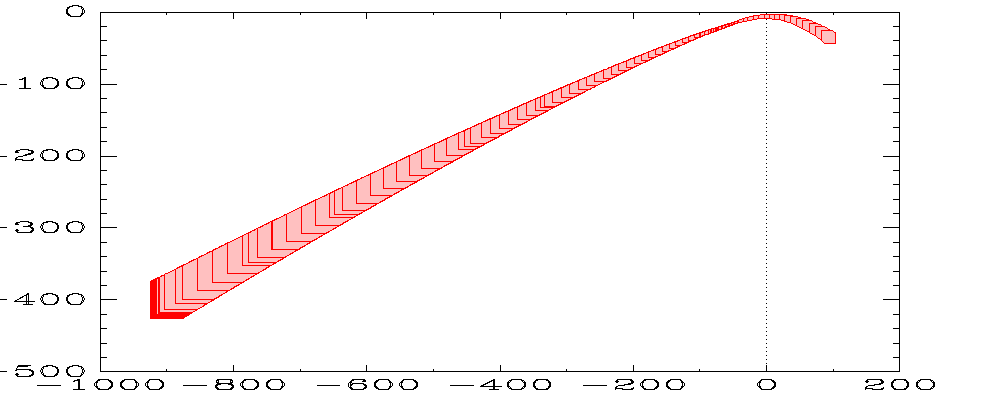
\includegraphics[width=0.9\columnwidth,trim=-7em 1em 7em 0, clip]{images/spaceex.png}
\subcaption{SpaceEx (continuous time)}%\label{fig:1c}
\end{minipage}
\\
\vspace{1em}
\begin{minipage}[b]{\linewidth}
  \centering
    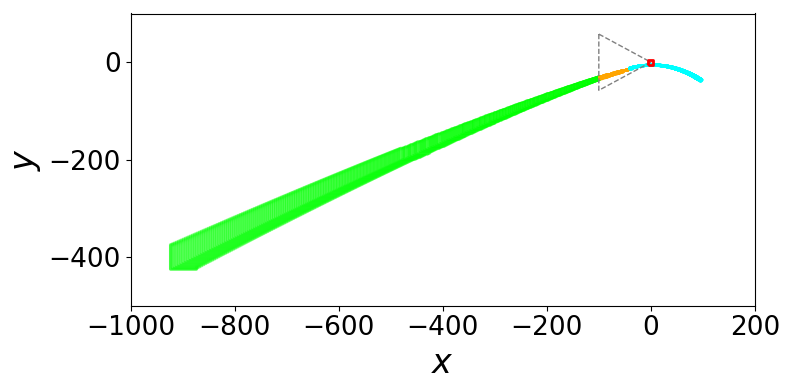
\includegraphics[width=0.9\columnwidth,trim=0 1.5em 0 0, clip]{images/step_d_0_25.png}
\subcaption{Our implementation (discrete time)}\label{fig:hylaa_qualitative}
\end{minipage}
\caption{The reachability plots using SpaceEx (top) in continuous time and our implementation based off Hylaa (bottom) in discrete time are qualitatively similar.
The initial states are in the lower left of the plots, the unsafe states are near the origin. In this plot, the switch to the passive mode occurs at exactly time 140.}\label{fig:qualitative}
\end{figure}

\subsection{SpaceEx}

We use the latest space-time clustering (STC) reachability method implemented in SpaceEx~\cite{frehse2013flowpipe} version \texttt{v0.9.8f}.
%
Two aggregation methods are available, \texttt{cull} (convex hull aggregation) and \texttt{none} (no aggregation).
%
We tune accuracy with the \texttt{flowpipe-tolerance} parameter as well as the number of support function directions to use, for which we consider
both \texttt{box} and \texttt{oct}.
%
By fixing the parameters, we can analyze the system as the passive-mode switch time parameter $r$ is increased from $0$ to $70$.
%
Since several options which trade off accuracy for computation time are available to the user, a fair comparison difficult.
%
We thus consider many permutations of these parameters, to try to find the best ones for each value of $r$.
%
In the experiments we had a one minute timeout to run the verification task.

With convex hull aggregation (Figure~\ref{fig:spaceex_chull}), the system can be analyzed successfully up to around $r=25$.
%
Some of the lines end before exceeding the timeout; these are the cases where increasing $r$ by 1 would prevent
successful analysis with those settings (safety could not be proven due to overapproximation).
%
Different accuracy settings can slightly go beyond this, with $r=30$ being possible in about one minute with \texttt{oct} directions and
\texttt{flowpipe-tolerance=0.01}.
%
This demonstrates the inherent overapproximation due to aggregation, where even modest uncertainty in the switch to the passive mode
prevents verification.

\begin{figure}[t]
\centerline{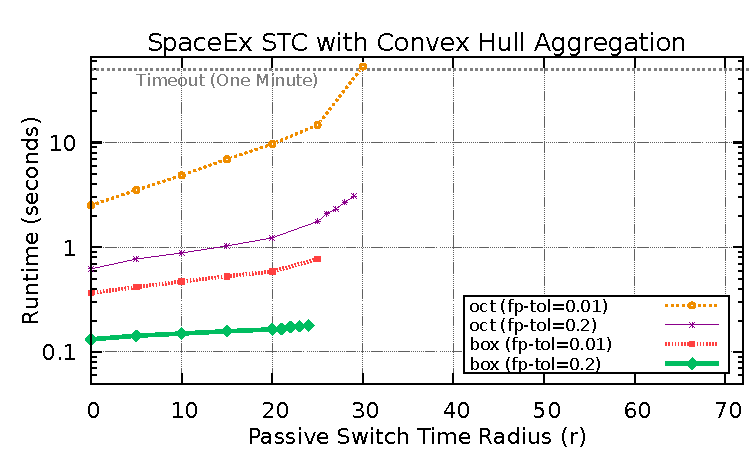
\includegraphics[width=0.9\columnwidth]{images/chull.pdf}}
\caption{SpaceEx with convex hull aggregation can analyze the system up to around $r=30$.}
\label{fig:spaceex_chull}
\end{figure}

With no aggregation (Figure~\ref{fig:spaceex_unagg}), we can be sure there is no error from aggregation overapproximation.
%
In this case, however, all combinations of mode-switching times along the execution path must be explored,
which can take excessive time when high accuracy settings are used.
%
In general, the number of possible switching times grows exponentially in the number of discrete transitions along system trajectories.
%
In this system, however, the longest path will only have two mode switches in the automaton in Figure~\ref{fig:ha}:
from mode 1 to mode 2, and mode 2 to the passive mode (the switch from mode 2 back to mode 1 is not executed for the given initial set).
%
Thus, unaggregated analysis is feasible.
%
In Figure~\ref{fig:spaceex_unagg}, SpaceEx can analyze the system up to around $r=55$ in this case.
%
It can still not do full uncertainty (up to $r=70$) since there is still some overapproximation from the choice of \text{flowpipe-tolerance} and the
choice of support function directions.
%
We did not find parameter values where we could analyze for much larger values of $r$ in a reasonable amount of time,
although theoretically analysis this should be possible by sufficiently increasing the accuracy settings.

\begin{figure}[t]
\centerline{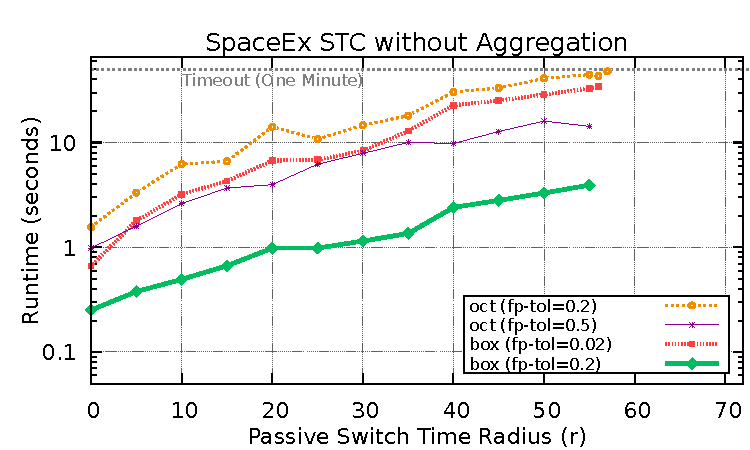
\includegraphics[width=0.9\columnwidth]{images/unagg.pdf}}
\caption{SpaceEx without aggregation can analyze the system up to around $r=55$.}
\label{fig:spaceex_unagg}
\end{figure}

One final note is that parameter selection is difficult for SpaceEx, and it would be unreasonable to perform an exhaustive search for every model
that needs analysis.
%
Although we have presented several reasonable options (and experimented with many others that were not presented), we have no guarantee that
the combinations of options we tried were the fastest or most accurate.
%
Further, there are other parameters we could have explored, such as the \texttt{lgg} reachability mode instead of \texttt{stc}, where a \texttt{clustering}
parameter is available to more finely control the aggregation process.
%
The SpaceEx help lists about 50 parameters, not all linked to method accuracy, that can affect the results of the computation,
and it can be difficult to select the correct ones to explore, even for people familiar with the verification algorithms.

\subsection{Proposed AGGDAG Approach}

Since the proposed aggdag method was implemented on top of the discrete-time Hylaa tool, care must be taken to ensure that a proper time step is chosen.
%
If the time step is too small, too many steps will be necessary and the analysis time can become excessive.
%
On the other hand, if the time step is too large, the unsafe states may be missed if they are reached between time steps
(this is called tunneling in collision detection methods).
%
We examine the reach set with switching time 140, which goes close to the unsafe states.

The analysis is shown in Figure~\ref{fig:step_size}.
%
This is zoomed-in plot of the system shown before from Figure~\ref{fig:hylaa_qualitative} near the unsafe states.
%
For the plot, it is clear that using a step size of 1.0 is unlikely to tunnel through the unsafe states,
although the smaller step size 0.25 may be preferred as the
reach set is a continuous set of state (the sets overlap between time steps).

\begin{figure}
\begin{minipage}[b]{\linewidth}
  \centering
  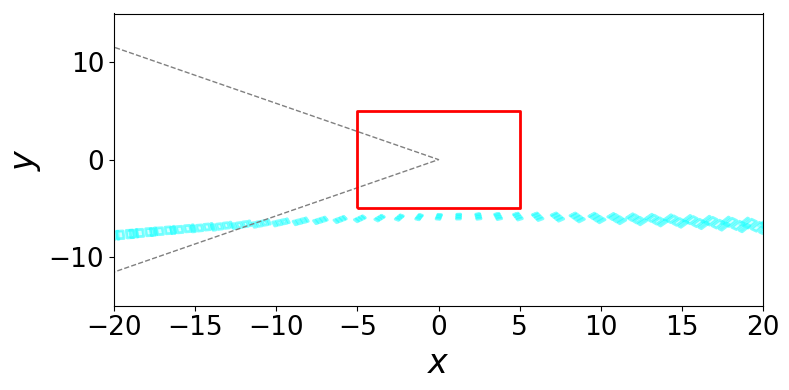
\includegraphics[width=0.9\columnwidth,trim=0 1.3em 0 0, clip]{images/step_a_1_0.png}
\subcaption{Step Size 1.0}%\label{fig:1a}
\end{minipage}%
\\
\vspace{1em}
\begin{minipage}[b]{\linewidth}
  \centering
    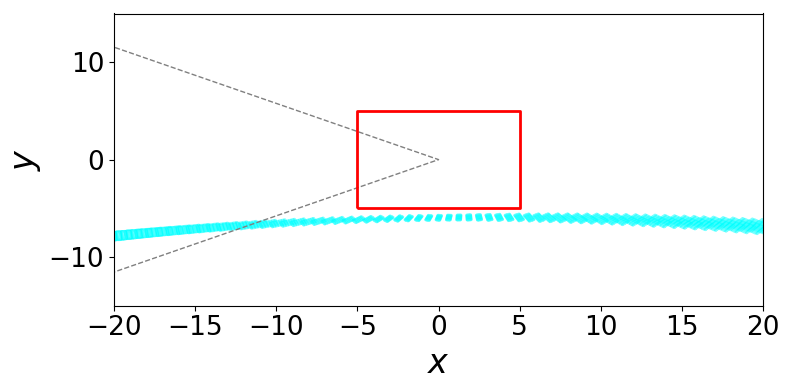
\includegraphics[width=0.9\columnwidth,trim=0 1.3em 0 0, clip]{images/step_b_0_5.png}
\subcaption{Step Size 0.5}%\label{fig:1b}
\end{minipage}
\\
\vspace{1em}
\begin{minipage}[b]{\linewidth}
  \centering
    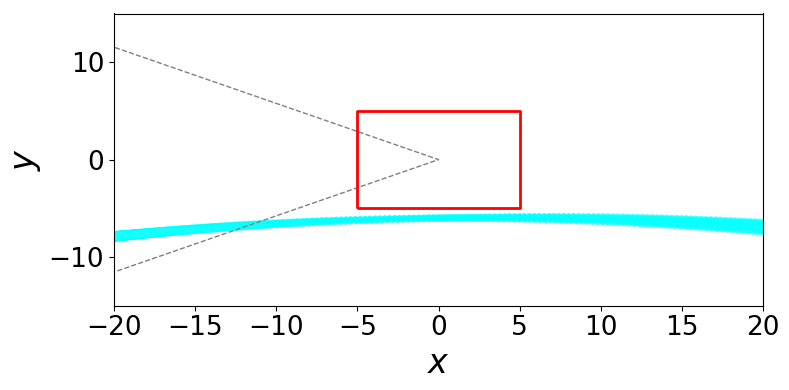
\includegraphics[width=0.9\columnwidth,trim=0 1.3em 0 0, clip]{images/step_c_0_25.png}
\subcaption{Step Size 0.25}%\label{fig:1c}
\end{minipage}
\\
\vspace{1em}
\begin{minipage}[b]{\linewidth}
  \centering
    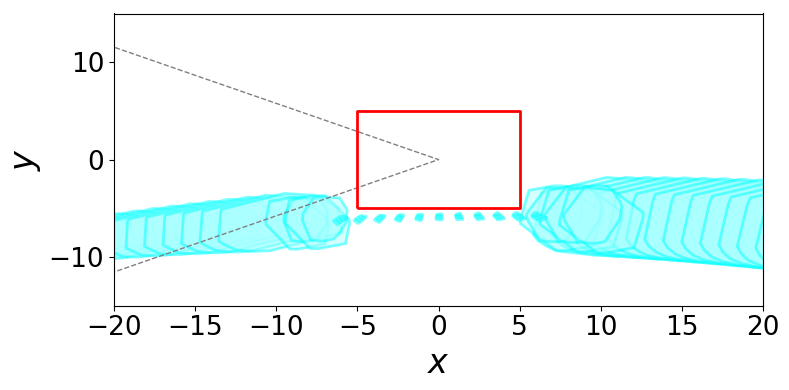
\includegraphics[width=0.9\columnwidth,trim=0 1.3em 0 0, clip]{images/deagg_1_0.png}
\subcaption{Deaggregation with Step Size 1.0}%\label{fig:1c}
\end{minipage}
\caption{Plots of the discrete-time reach set near the unsafe state are shown with aggregation disabled (top three plots).
  While a step size of 1.0 is unlikely to tunnel
  through the unsafe states (red box), using 0.25 provides a continuous set of reachable states. Our aggdag approach
  produces the bottom plot (step size 1.0), showing improved accuracy near the unsafe states using deaggregation.}\label{fig:step_size}
\end{figure}


We measure the performance of our method using all three step sizes.
%
The result is shown in Figure~\ref{fig:deagg}.
%
Since all three step sizes will deaggregate if an unsafe set is reached, the analysis is exact with respect to the specification.
%
This means that all the step sizes can successfully verify the system, even with maximum uncertainty in the switching time to the passive mode ($r = 70$).
%
The only difference is the performance of the methods.
%
In this case, all three step sizes verify the system before the one minute timeout.
%
Furthermore, parameter tuning with our approach is a bit more straightforward, as the main parameter is just the step size, and initial
analysis using simulations can be used to guide selecting a value for this.

\begin{figure}[t]
\centerline{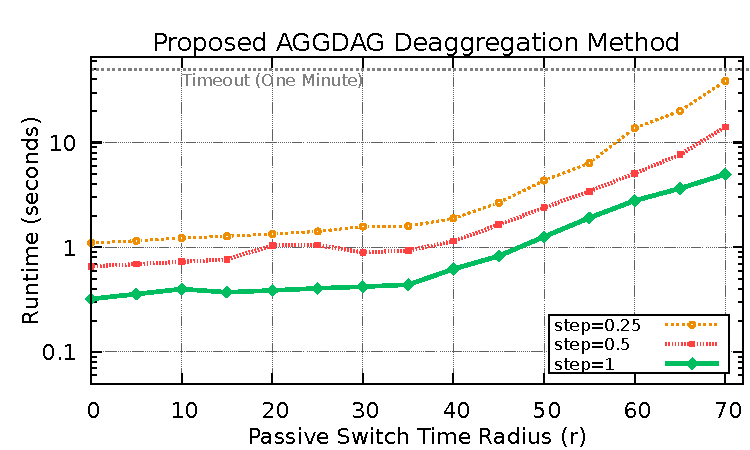
\includegraphics[width=0.9\columnwidth]{images/deagg.pdf}}
\caption{The proposed aggdag approach can analyze up to the full $r=70$, even for the smallest time step.}
\label{fig:deagg}
\end{figure}


A plot of the reachable state for the $r=70$ case is shown in Figure~\ref{fig:rendezvous}.
%
A video of the computation and refinement process is available at \url{https://gofile.io/?c=P0pKla}\footnote{We plan to replace
  anonymous links with youtube videos in the final version.}.
%
Prior to our analysis, we were unaware of any tool which could successfully analyzed this model in the complete passivity settings ($r=70$).

\begin{figure}[t]
\centerline{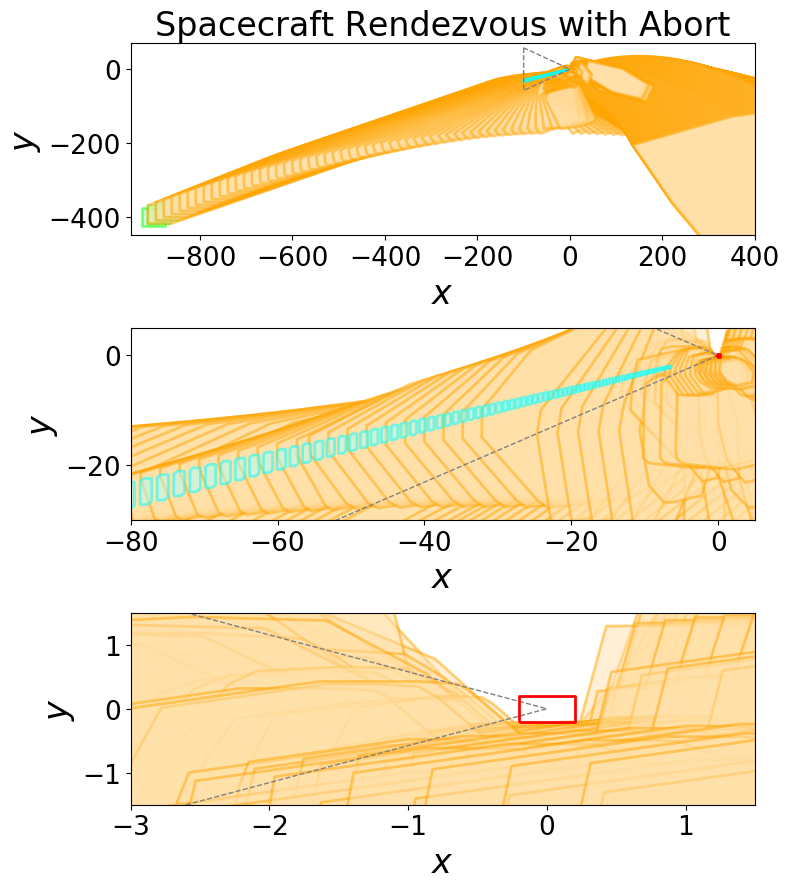
\includegraphics[width=0.8\columnwidth]{images/rendezvous.png}}
\vspace{-0.2cm}
\caption{{ The reachable set for the spacecraft rendezvous system at three different zoom levels is shown.
  Reachable states near the unsafe set (red square near origin) are deaggregated using the proposed approach until no unsafe states are reachable.
A video of the computation is online at \url{https://gofile.io/?c=P0pKla}.}}
\label{fig:rendezvous}
\end{figure}

